\begin{exercises} 
	\item A sailboat is sitting at rest near its dock.  A rope attached to the bow of the boat is drawn in over a pulley that stands on a post on the  end of the dock that is 5 feet higher than the bow.  If the rope is being pulled in at a rate of 2 feet per second, how fast is the boat approaching the dock when the length of rope from bow to pulley is 13 feet?
	
	\item A baseball diamond is a square with sides 90 feet long.  Suppose a baseball player is advancing from second to third base at the rate of 24 feet per second, and an umpire is standing on home plate.  Let  $\theta$ be the angle between the third baseline and the line of sight from the umpire to the runner.  How fast is $\theta$ changing when the runner is 30 feet from third base?
	
	\item Sand is being dumped off a conveyor belt onto a pile in such a way that the pile forms in the shape of a cone whose radius is always equal to its height.  Assuming that the sand is being dumped at a rate of 10 cubic feet per minute, how fast is the height of the pile changing when there are 1000 cubic feet on the pile?
	
	\item A swimming pool is 60 feet long and 25 feet wide. Its depth varies uniformly from 3 feet at the shallow end to 15 feet at the deep end, as shown in the Figure~\ref{F:3.5.Ez3}.
\begin{figure}[h]
\begin{center}
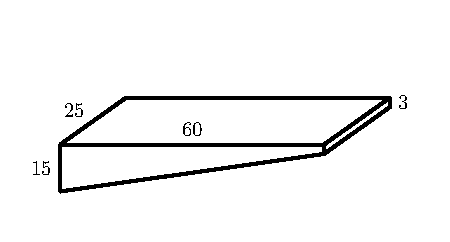
\includegraphics{figures/3_5_Ez3.eps}
\caption{The swimming pool described in Exercise 4.} \label{F:3.5.Ez3}
\end{center}
\end{figure}
Suppose the pool has been emptied and is now being filled with water at a rate of 800 cubic feet per minute. At what rate is the depth of water (measured at the deepest point of the pool) increasing when it is 5 feet deep at that end?  Over time, describe how the depth of the water will increase:  at an increasing rate, at a decreasing rate, or at a constant rate.  Explain.

\end{exercises}
\afterexercises